\chapter{Inprimakiak HTML5en}
\index{inprimakiak}\index{form}
HTML4 bertsioan inprimakiak programatzeko hainbat osagai bagenituen ere (\textit{input}, \textit{text}, \textit{numeric}, \textit{select}, \textit{checkbox}, \textit{radiobutton}…), HTML5ek osagai eta atributu berriak ekarri ditu: \index{placeholder}\textit{placeholder}, \index{autofocus}\textit{autofocus}, \index{email}\textit{email} eta \index{url} url —URLak sartzeko eremuak—, zenbakiak sartzeko eremuak (\index{spinbox}\textit{spinbox}, \index{slider}\textit{slider}), datak hautatzeko eremua, kolore bat hautatzeko eremua, bilaketak egiteko kutxak… Berritasun horiek guztiak gai honetan aztertuko dira.

HTMLn, oinarrizko inprimaki baten itxura honakoa da:

\begin{lstlisting}[language=JavaScript]
<form name="inprimakia" action="/kudeatzailea">
   Izena: <input type="text">
   <br><input type="submit">
</form>
\end{lstlisting}


HTML4 bertsioan, inprimakietan erabil zitezkeen eremu motak \ref{tab:my-table}.  taulan zehazten dira.

\begin{table}[]
\resizebox{\textwidth}{!}{% use resizebox with textwidth
\begin{tabular}{lll}
\multicolumn{1}{c}{\textbf{Eremu mota}} & \multicolumn{1}{c}{\textbf{HTML kodea}}                           & \multicolumn{1}{c}{\textbf{Iruzkinak}}             \\ \hline
Kontrol-laukia                          & \textless{}input type="checkbox"\textgreater{}                    & gaitu eta desgaitu daiteke                         \\
Aukera-botoia                           & \textless{}input type="radio"\textgreater{}                       & multzokatu egiten dira                             \\
Pasahitza-eremua                         & \textless{}input type="password"\textgreater{}                    & puntuak idatziko ditu edozein tekla sakatzean \\
Aukera-zerrenda                         & \textless{}select\textgreater{}\textless{}option\textgreater{}... &            \textit{combobox} izenarekin ere ezagutzen dira                                        \\
Fitxategi-eremua                        & \textless{}input type="file"\textgreater{}                        & disko gogorretik fitxategi bat hautatzeko eremua                    \\
Bidaltzeko botoia                       & \textless{}input type="submit"\textgreater{}                      & submit botoia sakatuko dugu inprimakia bidaltzeko \\
Testu-eremua                            & \textless{}input type="text"\textgreater{}                        &            gehien erabiltzen den eremu mota                                        \\ \hline
\end{tabular}
}
\caption{HTML4 bertsioan inprimakietan erabil zitezkeen zenbait eremu mota.}
\label{tab:my-table}
\end{table}

Noski, eremu horiek HTML5en ere erabil daitezke, baina bertsio berri honetan beste eremu mota batzuk sartu ziren, atal honetan aztertuko ditugunak.

\section{Eremu eta atributu berriak HTML5en}

Banan-banan hurrengo atributu eta funtzionalitate berriak landuko ditugu:

\begin{enumerate}
    \item placeholder
    \item autofocus
    \item email eta URLak sartzeko eremuak 
    \item zenbakiak (\textit{spinbox}, \textit{slider})
    \item data bat hautatzeko eremua 
    \item kolore bat hautatzeko eremua 
    \item bilaketak egiteko kutxak 
    \item derrigorrezko eremuak 
    \item inprimakien baliozkotzea
\end{enumerate}

\subsection{Placeholder atributua}
 
 Testu-eremu batean sar daitekeen testu adibide bat bistaratzeko atributua da \textit{placeholder} (ikus \ref{fig:placeholder}. irudia). Adibidez:
 
 \begin{lstlisting}[language=JavaScript,numbers=none]
 <form>
    <input name="q" placeholder="Zure izena">    
    <input type="submit" value="Bidali">
</form>
 \end{lstlisting}
 
 \begin{figure}[ht]
	\centering
\begin{tikzpicture}
\node[anchor=south west,inner sep=0] (image) at (0,0)
   {
\includegraphics[trim=0cm 0cm 0cm 0cm, clip=true, width=0.5\textwidth]{img/placeholder.png}};
\end{tikzpicture}
\caption{\textit{Placeholder} atributu motaren adibidea.}
\label{fig:placeholder}
\end{figure}

 \subsection{Autofocus atributua}
 \textit{Autofocus} atributuak duen eremuak fokua hartuko du orria kargatzen denean. Adibidez, google.com kargatzean zuzenean idatz dezakezu bilatu nahi duzuna, inongo eremuan klik egin gabe, bilaketaren testua idazteko eremuak \textit{autofocus} atributua gaituta duelako.
 
 \begin{lstlisting}[language=JavaScript,numbers=none]
 <form>
  <input name="q" autofocus>
  <input type="submit" value="Search">
</form>
 \end{lstlisting}
 
 \subsection{Email eremu mota}
 
 Email eremu mota (\ref{fig:emailmota}. irudia) testu-eremu motakoa bezalakoa da, berezitasun pare batekin: 
 
 \begin{itemize}
     \item Android eta iOS sistema eragileetan teklatu mota aldatzen da bertan klik egitean.
     \item Nabigatzaile batzuek egiaztapen automatikoak egiten dituzte (helbide elektroniko zuzena dela egiaztatzeko).
 \end{itemize}

 \begin{lstlisting}[language=JavaScript,numbers=none]
 <form>
  <input type="email">
  <input type="submit" value="Go">
</form>
\end{lstlisting}
 
 \begin{figure}[ht]
	\centering
\begin{tikzpicture}[framed]
\node[anchor=south west,inner sep=0] (image) at (0,0)
   {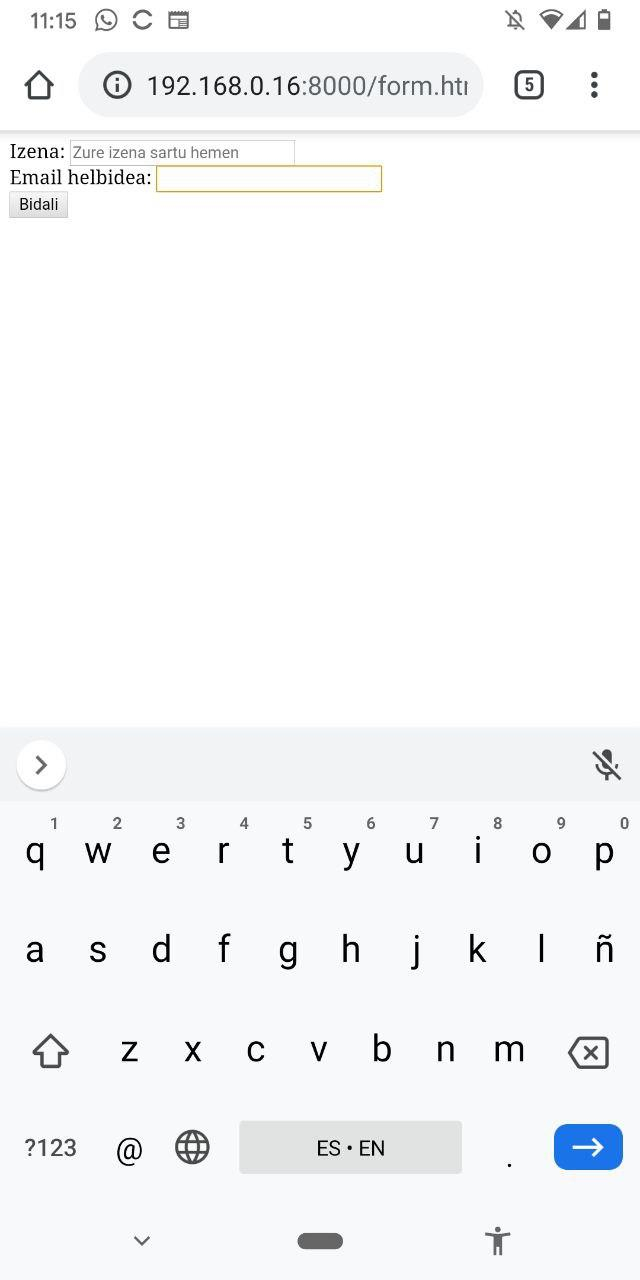
\includegraphics[trim=0cm 0cm 0cm 0cm, clip=true, width=0.25\textwidth]{img/email.jpg}};
   \draw [draw=red] (0.70,0.70) rectangle ++(0.3,0.3);
\end{tikzpicture}
\caption{Email motako eremu batean sakatzean, mugikorretan irekitzen den teklatuan, @ karaktereak berezko tekla izango du (testu arruntetan \textit{emojiak} idazteko okupatzen duen tekla).}
\label{fig:emailmota}
\end{figure}

 \begin{figure}[ht]
	\centering
\begin{tikzpicture}[framed]
\node[anchor=south west,inner sep=0] (image) at (0,0)
   {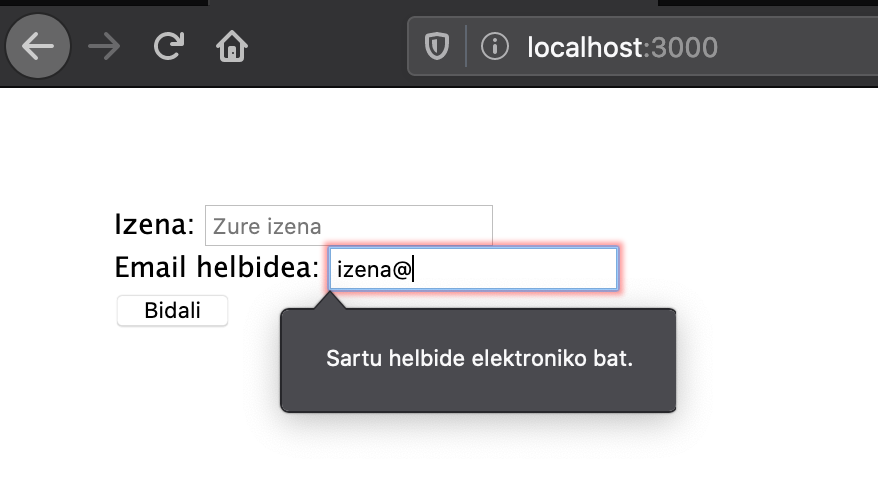
\includegraphics[trim=0cm 0cm 0cm 0cm, clip=true, width=0.75\textwidth]{img/firefoxemailfield.png}};
\end{tikzpicture}
\caption{Nabigatzaileek automatikoki egiaztatzen dute email zuzen bat sartu dela email motako eremu batean.}
\label{fig:emailmota}
\end{figure}

\subsection{URL eremu mota}

URL eremu mota URLak sartzeko erabiliko dugu (adibidez, https://domeinua.eus).
Nabigatzaileak automatikoki egiaztatuko du benetan URL bat dela, hainbat arau betetzen dituela baieztatuz (barra bat / agertzen dela, gutxienez puntu bat, ez duela zuriunerik...)


\subsection{Zenbakiak sartzeko eremuak: \textit{range}, \textit{slider} eta \textit{spinbox} eremu motak}

Zenbakiak \hl{text} edo \hl{range} motako eremuak erabiliz sar daitezke. \index{range}\textit{Range} eremu motan \ref{fig:rangeeremumota}. irudian bistaratzen den bezalako osagai bat izango dugu. Osagai horri \index{slider} \textit{slider} ere esaten zaio. Beste eremu mota bat zenbakiak sartzeko \index{number}\textit{number}  izenekoa da. Mota horri, berriz, \index{spinbox}\textit{spinbox} ere esaten zaio. Bertan soilik zenbakiak sar daitezke eta gezien bidez zenbakia handitu edo gutxitu egin daiteke. Zenbakien arteko jauzia ere kontrola daiteke \index{step}\textit{step} atributuarekin (ikus \ref{fig:numbereremumota} irudia).


 \begin{figure}[ht]
	\centering
\begin{tikzpicture}[framed]
\node[anchor=south west,inner sep=0] (image) at (0,0)
   {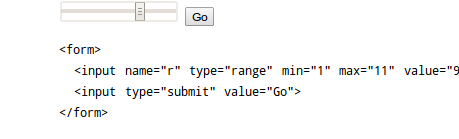
\includegraphics[trim=0cm 0cm 0cm 0cm, clip=true, width=0.75\textwidth]{img/range.png}};
\end{tikzpicture}
\caption{\textit{Range} eremu mota.}
\label{fig:rangeeremumota}
\end{figure}

 \begin{figure}[ht]
	\centering
\begin{tikzpicture}[framed]
\node[anchor=south west,inner sep=0] (image) at (0,0)
   {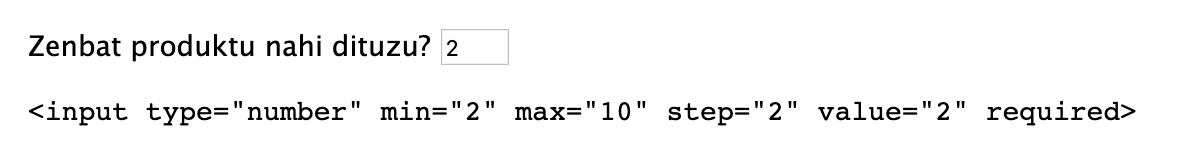
\includegraphics[trim=0cm 0cm 0cm 0cm, clip=true, width=0.75\textwidth]{img/spinbox.png}};
\end{tikzpicture}
\caption{\textit{Number} (edo \textit{spinbox}) eremu mota.}
\label{fig:numbereremumota}
\end{figure}


\subsection{Datak sartzeko eremuak}

 HTML4 bertsioan ez zegoen eremu zehatzik datak sartzeko inprimaki batean; izan ere, JavaScript liburutegi ezberdinak sortu ziren arazo hori konpontzeko (adibidez, \href{https://jqueryui.com/datepicker/}{jQuery DatePicker}\footnote{https://jqueryui.com/datepicker/}). HTML5en, berriz, hainbat osagai ditugu datak eta orduak hautatzeko (\ref{fig:datakorduak}. irudia).
 
 
 \begin{figure}[ht]
	\centering
\begin{tikzpicture}
\node[anchor=south west,inner sep=0] (image) at (0,0)
   {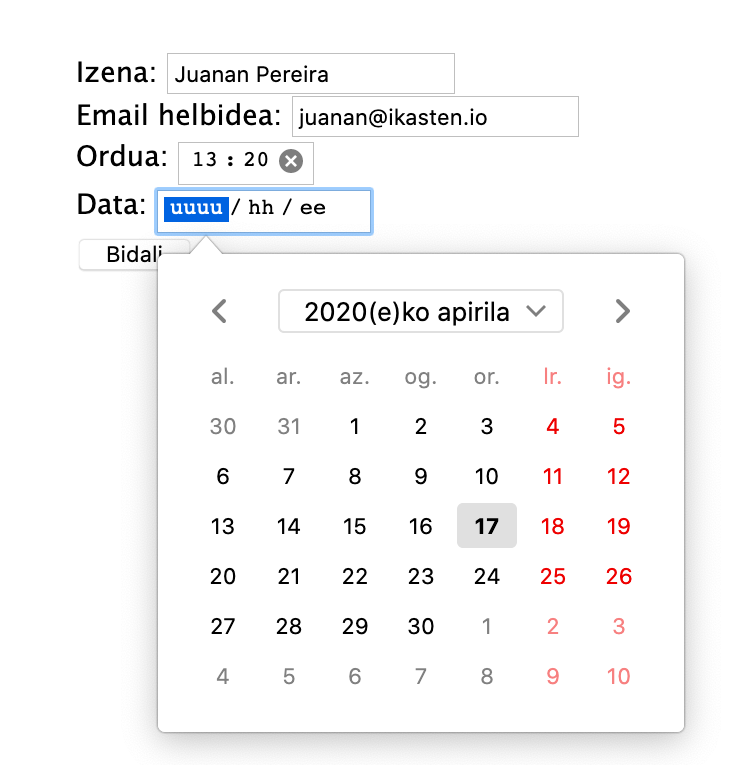
\includegraphics[trim=0cm 0cm 0cm 0cm, clip=true, width=0.65\textwidth]{img/dataetaorduak.png}};
\end{tikzpicture}
\caption{Data eta orduak hautatzeko eremuak.}
\label{fig:datakorduak}
\end{figure}

\subsection{Kolore bat hautatzeko eremu mota}
Kolorea hautatzeko eremua ere berria da HTML5en. Eremuaren izena erraza da: \index{color}\textit{color}. Besterik ezeko balio bat ere eman diezaiokegu. Kolorearen balioa RGB (\textit{red,green,blue}) erabiliz edo zuzenean izen bat esleituz ezar daiteke. Alegia, kolorearen izena gorria bada, \textit{red} izena erabil dezakegu edo haren baliokidea RGB formatuan ``\#ff0000''. 

\index{RGB}RGB formatuak hiru osagai zehazten ditu: gorria, berdea eta urdina koloreen balioak, sistema hamaseitarrean. Berdea adierazteko, adibidez, ``\#00ff00'' erabiliko genuke (edo \hl{ff} baino txikiagoa den beste balio bat berde apalago bat hautatzeko). Noski, oinarrizko koloreak nahastu egin daitezke beste kolore batzuk lortzeko. Adibidez, morea lortzeko kolorea honakoa litzateke: \#ff40ff. Dena den, sistema eragileak berak  \textit{pantone} bezalako kontrol bat eskaintzen du, kolorea grafikoki hautatu ahal izateko, zenbakiak zeintzuk diren jakin gabe (ikus \ref{fig:colorinput} irudia).

\begin{figure}[ht]
	\centering
\begin{tikzpicture}
\node[anchor=south west,inner sep=0] (image) at (0,0)
   {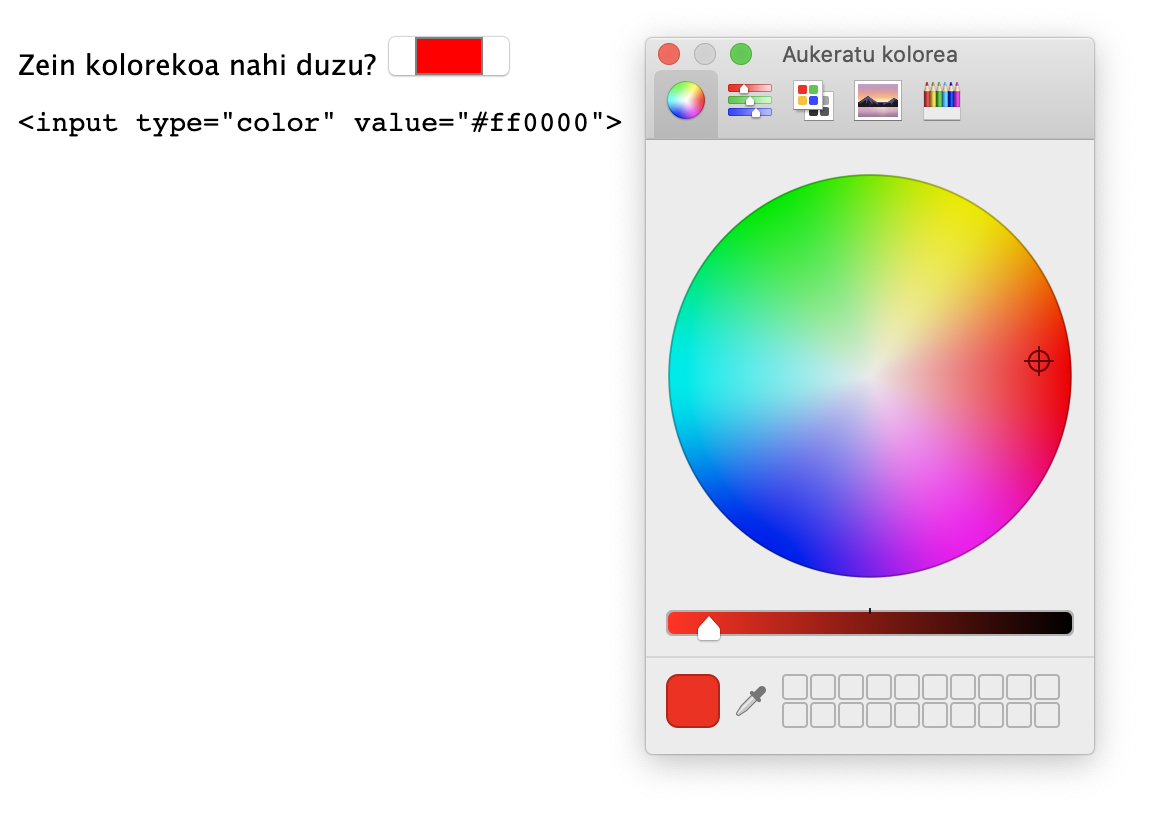
\includegraphics[trim=0cm 0cm 0cm 0cm, clip=true, width=0.65\textwidth]{img/colorinput.png}};
\end{tikzpicture}
\caption{Koloreak hautatzeko \textit{color} eremu mota erabiliko dugu.}
\label{fig:colorinput}
\end{figure}

\subsection{Bilaketak egiteko \textit{search} eremuak}
Bilaketak egiteko \index{search}\textit{search} motako \textit{<input>} osagaiak testu-eremu arruntak bezalakoak dira, erabiltzaileak bertan kontsultak eta bilaketen testua idazteko diseinatuak. Bisualki, berriz, berezitasunak izan ditzake, batez ere mugikorretan bistaratzen badira. Adibidez, Android sistema eragileak lupa baten ikurra jarriko dio Enter teklari (ikus \ref{fig:searchinput}. irudia).

\begin{figure}[ht]
	\centering
\begin{tikzpicture}[framed]
\node[anchor=south west,inner sep=0] (image) at (0,0)
   {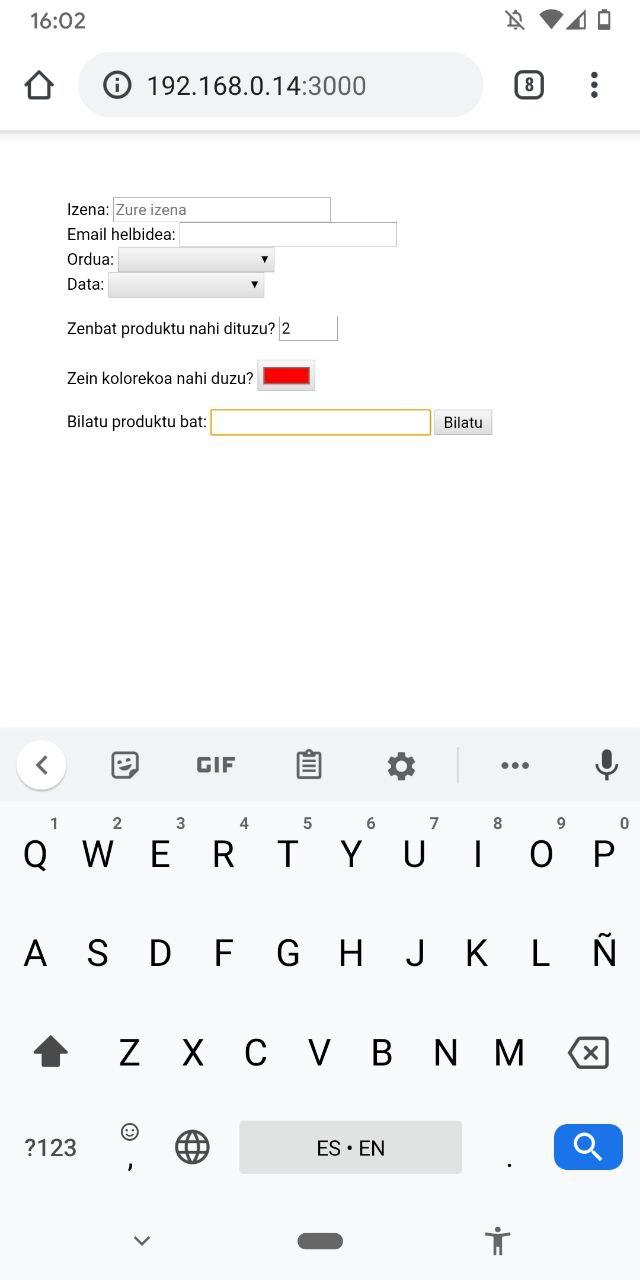
\includegraphics[trim=0cm 0cm 0cm 0cm, clip=true, width=0.35\textwidth]{img/searchinput.jpg}};
    \draw [draw=red] (4.95, 0.90) rectangle ++(0.8,0.6);
\end{tikzpicture}
\caption{\textit{Search} eremu motak lupa baten ikurra erabiliko du \textit{Enter} teklan, mugikor batetik bistaratzean.}
\label{fig:searchinput}
\end{figure}

\subsection{Derrigorrezko eremuak (\textit{required})}

\textit{Color} eremu motak aztertzean, \textit{<input>} osagaian \index{required}\hl{required} atributua ikus dezakegu (\ref{fig:colorinput}. irudia). Eremu horretan erabiltzaileak zerbait aukeratu behar duela esan nahi du \textit{required} horrek. Ez badu horrela egiten, nabigatzaileak errore bat jaurtiko du inprimakia bidaltzeko botoian sakatzean eta ez digu bidaltzen utziko arazoa konpondu arte.

\subsection{Inprimakien baliozkotzea}

Inprimaki bat bidaltzean, derrigorrezko (\textit{required}) eremuez gain, eremuen balioak egiaztatu behar dira inprimakia zerbitzarira bidali baino lehen. Eremu jakin batzuen balioa automatikoki konprobatuko da (adibidez, email motakoak, \ref{fig:emailmota}. irudian ikusten den bezala). Beste elementu batzuen balioa, ordea, skript baten bidez egiaztatu beharko ditugu. Adibidez, demagun \ref{fig:datakorduak}. irudian data eta ordu bat hautatzean, erabiltzaileak soilik lanegunak direnak aukeratu ditzakeela, eta soilik 10:00-14:00 ordu-tartean. Aukeraketa hori zuzena ez bada, errore-mezu bat pantailaratuko dugu, arrazoia azalduz.

Kodea \ref{lst:inprimakiaegiaztatu}. listatuan aurkezten da. Bertan \textit{form} etiketari \index{onsubmit}\textit{onsubmit} kudeatzaile bat esleitu zaio. Kudeatzaile horrek boolear bat bueltatu behar du: dena ondo badago inprimakian,  \textit{true} (eta inprimakia zerbitzarira bidaliko da, haren \textit{action} atributua zehazten duen helbidera), eta erroreren bat aurkituz gero, \textit{false} (eta, beraz, ez da inprimakia zerbitzarira bidaliko).

\begin{figure}[ht]
	\centering
\begin{tikzpicture}[framed]
\node[anchor=south west,inner sep=0] (image) at (0,0)
   {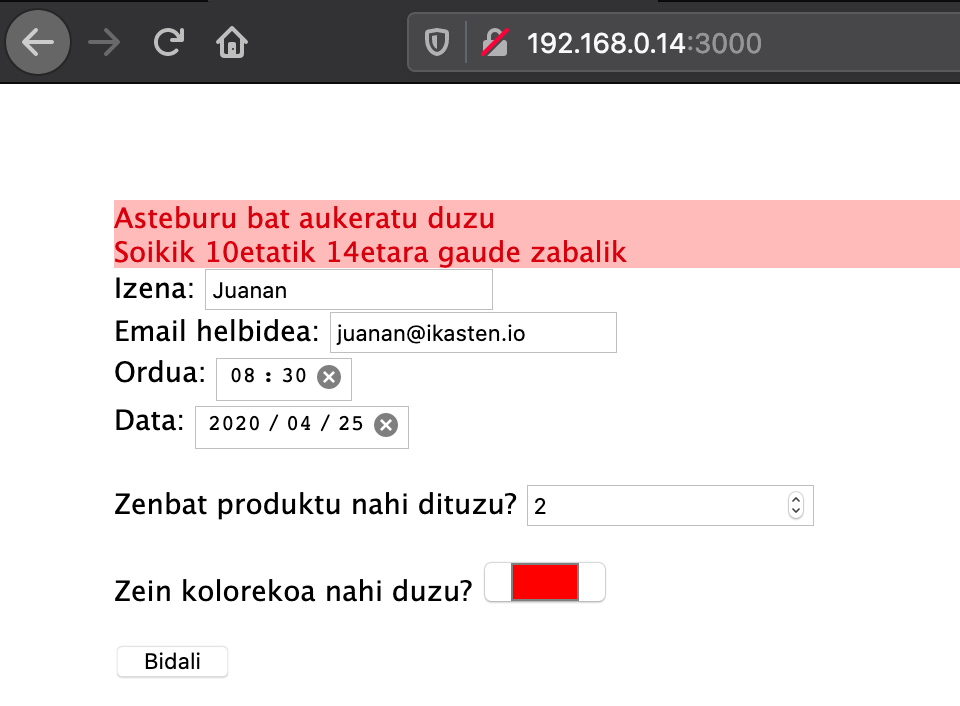
\includegraphics[trim=0cm 0cm 0cm 0cm, clip=true, width=0.5\textwidth]{img/formegiaztatu.png}};
\end{tikzpicture}
\caption{Inprimaki baten balioak egiaztatu ondoren errore bat pantailaratu dezakegu beharrezkoa bada.}
\label{fig:searchinput}
\end{figure}

\clearpage
%\begin{minipage}[t][.8\textheight][s]{\textwidth}
\begin{lstlisting}[language=JavaScript,caption={Inprimaki baten balioak egiaztatzeko kodea.},captionpos=b]
<script>
    function egiaztatu(){
        const inprimakia = document.getElementById('inprimakia');
        // ordua:minutua formatuan dagoen string batetik ordua lortu
        const ordua = inprimakia.ordua.value.split(":")[0];
        // eguna lortu (string bat date datu motan bihurtu)
        const eguna = new Date(inprimakia.data.value);
        let erroreak = '';
        // 6 = larunbata 0 = igandea 1 = astelehena ...
        if (eguna.getDay() == 6 || eguna.getDay() == 0) {
            erroreak += 'Asteburu bat aukeratu duzu';
        }
        // ordua 10-14 tartean egon behar da
        if (ordua < 10 || ordua > 14) {
            erroreak += '<br>Soikik 10etatik 14etara gaude zabalik';
        }
        if (erroreak != ''){
            document.getElementById('erroreak').innerHTML = erroreak;
            return false;
        }
        return true;
    }
</script>
</head>
<body>

<div id="erroreak"></div>
<form id="inprimakia" method="POST" action="/inprimakia" onsubmit="return egiaztatu();" >
\end{lstlisting}
\label{lst:inprimakiaegiaztatu}
%\end{minipage}

\section{Ariketak}

Sor ezazu \ref{fig:inprimakiak}. irudian dagoen inprimakia HTML5ek eskaintzen dituen eremu berriak erabiliz eta honako arauak kontuan hartuz:

\begin{figure}[ht]
	\centering
\begin{tikzpicture}[framed]
\node[anchor=south west,inner sep=0] (image) at (0,0)
   {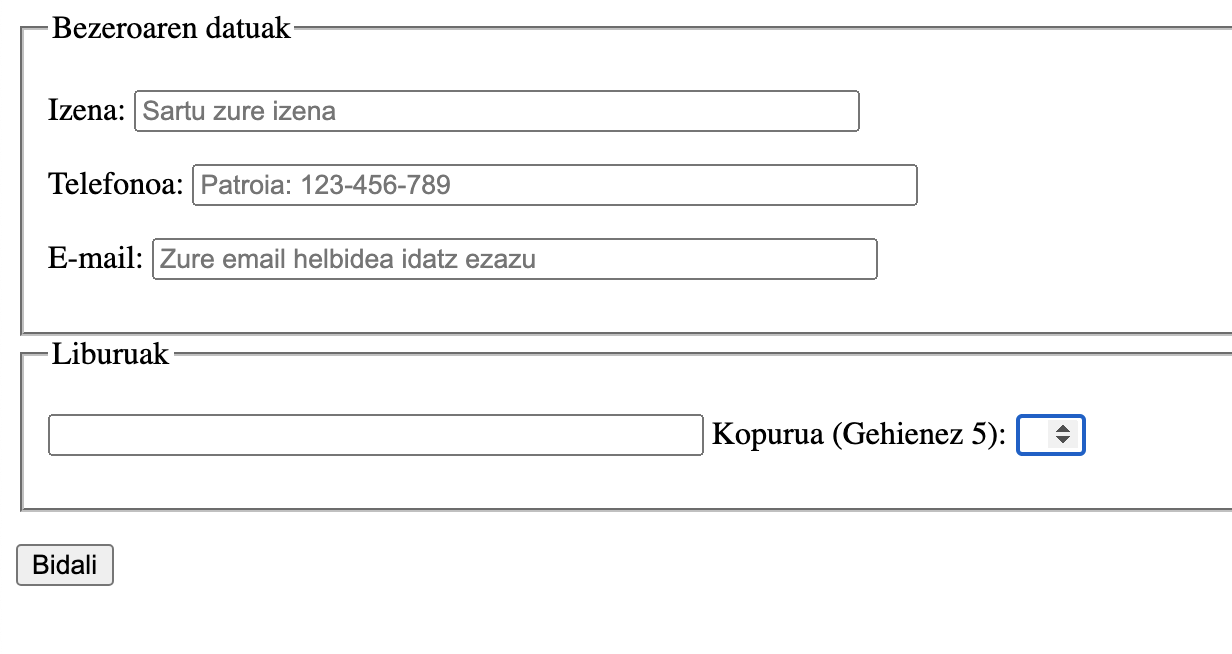
\includegraphics[trim=0cm 0cm 0cm 0cm, clip=true, width=0.5\textwidth]{img/inprimakiak/inprimakia.png}};
\end{tikzpicture}
\caption{Erabiltzaileak datuak idatzi ostean \textit{Bidali} botoian  sakatuko du. Akatsik balego, jakinaraziko zaio.}
\label{fig:inprimakiak}
\end{figure}

\begin{itemize}
    \item Izena eremuak orria kargatzean fokua hartu behar du.

\item Telefonoa eremua ez da orain arte agertu, baina gai
izango zinateke programatzeko? Eta telefono baten
patroia automatikoki antzemateko? (Argibidea: ikus \textit{regex} patroiak
HTML5en)

\item Ohart zaitez eremu batzuetan txantiloi gisa zerbait agertzen dela aurreidatzita (\textit{placeholder} bat).

\item Liburuak izeneko eremuan klik bikoitza egitean 5 libururen izenak agertu behar dira (ikus \textit{Datalist} HTML5en).
\end{itemize} 